\documentclass{article}
\usepackage{enumitem}
\usepackage{graphicx}
\usepackage{grffile}
\usepackage{float}
\begin{document}
\title{%
 Deliverable 1\\
 \large An identification of problems, derivation of high level requirements\\
 \large and an articulation of features using controlled notation
}
\author{Epic Group}
\date{}
\maketitle

\section*{Introduction}
The purpose of this report is to identify and express high level requirements
regarding a potential software system via structured notation. We will express
the contents of our report in the following format.
\begin{enumerate}
\item \textbf{Problem Statements}: A series of problem statements which will
investigate a number of problems we will solve via our software prototype.
\item \textbf{User Stories}: An idenfitication of features based on the problem
statement previously specified.
\item \textbf{Low-Fidelity Prototype}: A paper physical sketch of the UI 
elements integrated with a storyboard-like chronological script.
\item \textbf{High-Fidelity Prototype}: A computerised render of the
low-fidelity prototype previously specified.
\end{enumerate}
Our report will strictly harbor to controlled software engineering notation, 
such as the utilisation of user stories and Connextra notation.
\section{Problem Statements}
We will enumerate over a series of problem statements tangibly solved by
software to be resolved in our prototype.

\subsection{Restricted Database Problem Statement}
Contemprorary internet recommendation algorithms are typically a smaller
software component of a larger media streaming or distribution service,
restricting the scope of recommendation to media within such a service.
\subsection{Speculative Result Problem Statement}
Current media recommendation services typically infer recommendations based
on the initial media consumption habits of its users. Consequently,
the resultant recommendations are implicly obtained and therefore unreliable
and largely erroneous.
\subsection{Cheap Implementation Problem Statement}
The computational requirements of competing recommendation algorithms are
often minimised in order to mitigate the resource load on a multifaceded
service which also provides streaming or forum capabilities.
\subsection{User Requrement Problem Statement}
Database leaks are prevalent and inevitable, and any service which needlessly
requires user account creation risks fracturing the privacy and trust of its
user base upon such a database breach.
\subsection{User Input Sanitisation Problem Statement}
Contemporary internet recommendation algorithms rely solely on the input
of its user base in providing results, enabling the possibility of malicious
actors explotiting the system to redirect users to dangerous or illicit content.
\subsection{Corporate Bias Problem Statement}
Due to the for-profit nature of widely used media recommendation algorithms,
results are often skewed towards benefiting publishers who can afford to
partner with media recommendation service providers.

\section{High Level Requirements and Features}
\begin{enumerate}
\item
\textbf{High Level Requirement}: An unrestricted, encompassing movie database.
\newline
\textbf{Feature}: An IMDb (Internet Movie Database) and OMDb (Open Movie 
Database) sourced database.
\newline
\textbf{User Story}: As an avid film watcher, I want to receive tailored, 
specific recommendations relevant to me.
\newline
\textbf{Scenario}:
Given that I am on the website and that I perform a movie search, when I recieve
results, then I should see results which are most relevant to me.
\newline

\item
\textbf{High Level Requirement}: An explicitly obtained search profile.
\newline
\textbf{Feature}:
The serving of a procedurally generated series of questions based solely on the
reponses of the current session.
\newline
\textbf{User Story}:
As someone who enjoys multiple movie genres, I want to recieve recommendations
which are not based on my previous viewing sessions.
\newline
\textbf{Scenario}:
Given that I am on the website and I have previously made a search and I 
perform a new search, when I recieve results, then the results should not be
an amalgamation of my previous sessions.
\newline

\item
\textbf{High Level Requirement}: Unlimited movie search sessions.
\newline
\textbf{Feature}:
Untracked user sessions; sessions are tracked only via the client.
\newline
\textbf{User Story}:
As a power user, I wish to be able to receive many movie recommendations over
a short period of time.
\newline
\textbf{Scenario}:
Given that I have performed many searches recently, and I want to perform a new
search, when I recieve results, then the new results are not rate limited.
\newline

\item
\textbf{High Level Requirement}: Non compulsary user account creation.
\newline
\textbf{Feature}:
An accountless search ability.
\newline
\textbf{User Story}:
As a first time website visiter, I wish to be able to perform a search without 
offering my credentials and other personal information to first generate an 
account.
\newline
\textbf{Scenario}:
Given that I have visited the website, and I want to make my first search, when
I attempt to search, then I am not prompted to first create an account.
\newline

\item
\textbf{High Level Requirement}: No user input effect on database.
\newline
\textbf{Feature}:
Complete sourcing of database information from a single, immutable authority.
\newline
\textbf{User Story}:
As a user of the service, I wish to be able to use the service in its full 
capability without malicious content from ever corrupting my movie suggestions.
\newline
\textbf{Scenario}:
Given that I have visited the website, and I make my search, when I receive my
results, then the results should be free from user generated content.
\newline

\item
\textbf{High Level Requirement}: No corporate influence on recommendations.
\newline
\textbf{Feature}:
A keyword based search mechanism.
\newline
\textbf{User Story}:
As a user of the service, I do not wish to recieve recommendations based on
corporate interests or monetary influence.
\newline
\textbf{Scenario}:
Given that I have visited the website, and I make my search, when I receive my
results, then the results should be free from corporate bias.
\newline
\end{enumerate}

\section{Low-Fiedelity Prototype}
The following images are rough sketches of a potential final website design.
\subsection{Landing Page}
\begin{figure}[H]
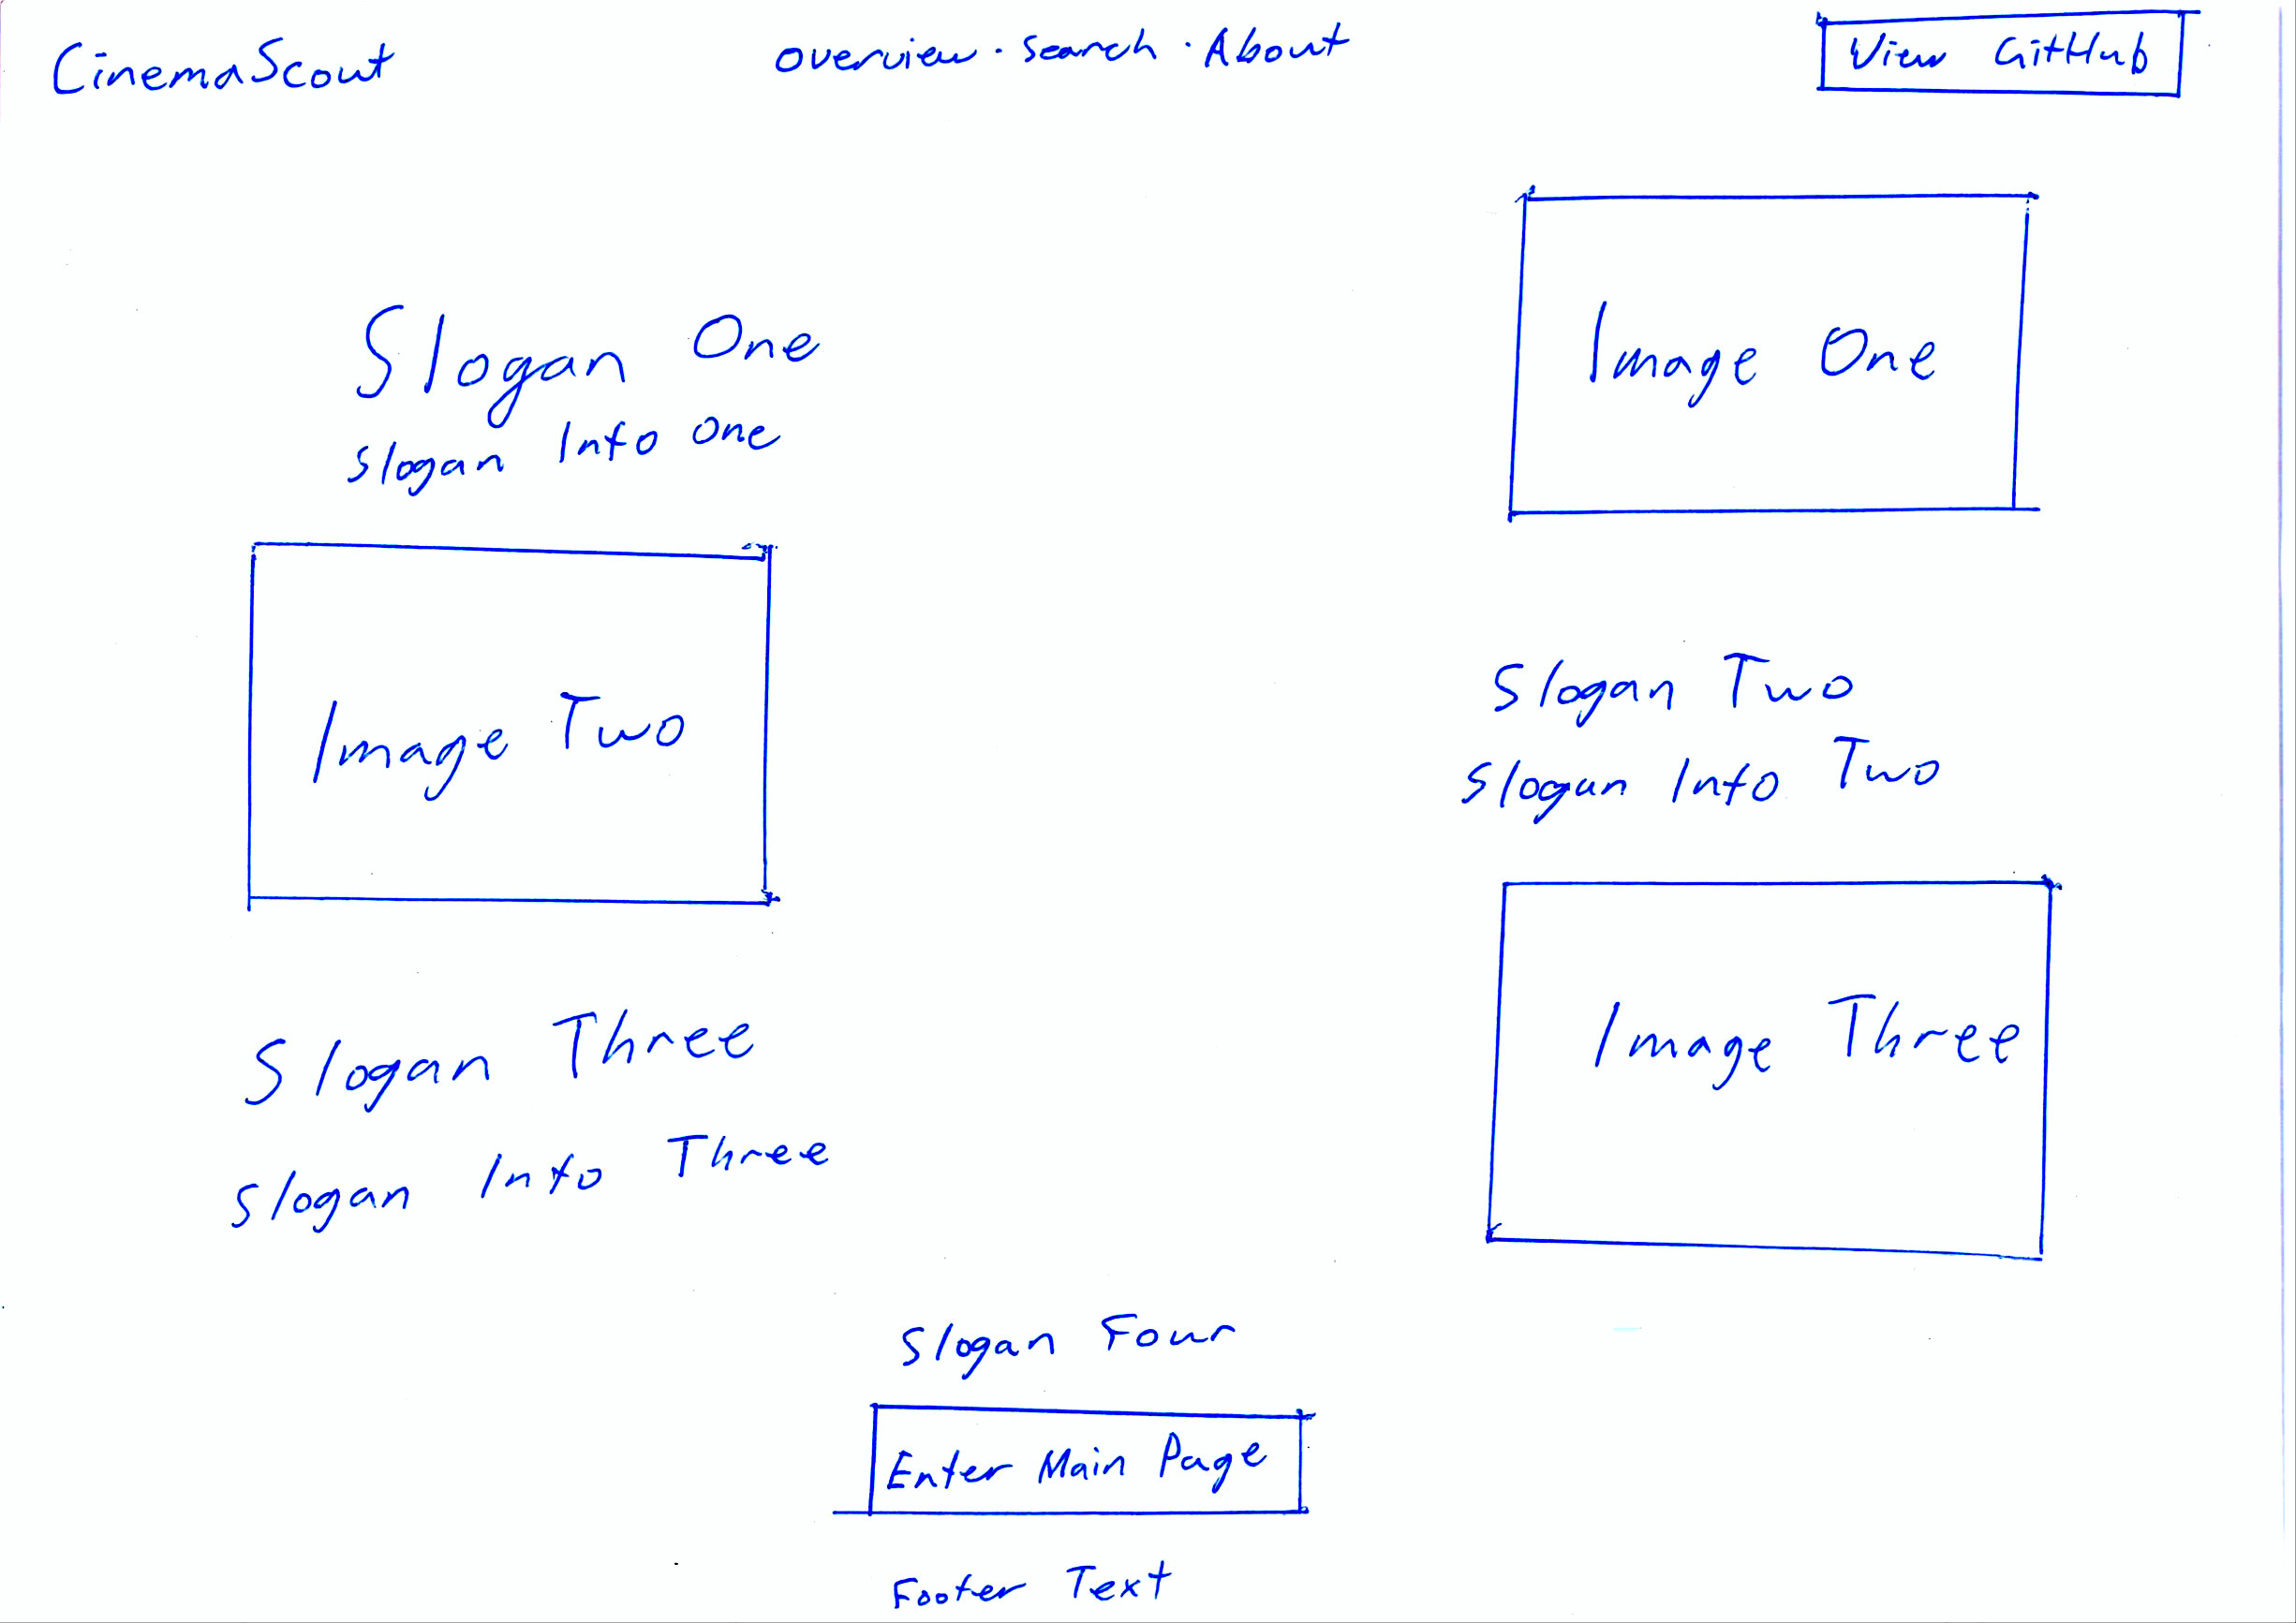
\includegraphics[width=\columnwidth]{res/landing.jpg}
\caption{Rough sketch of the landing page.}
\end{figure}
\subsection{Search Page}
\begin{figure}[H]
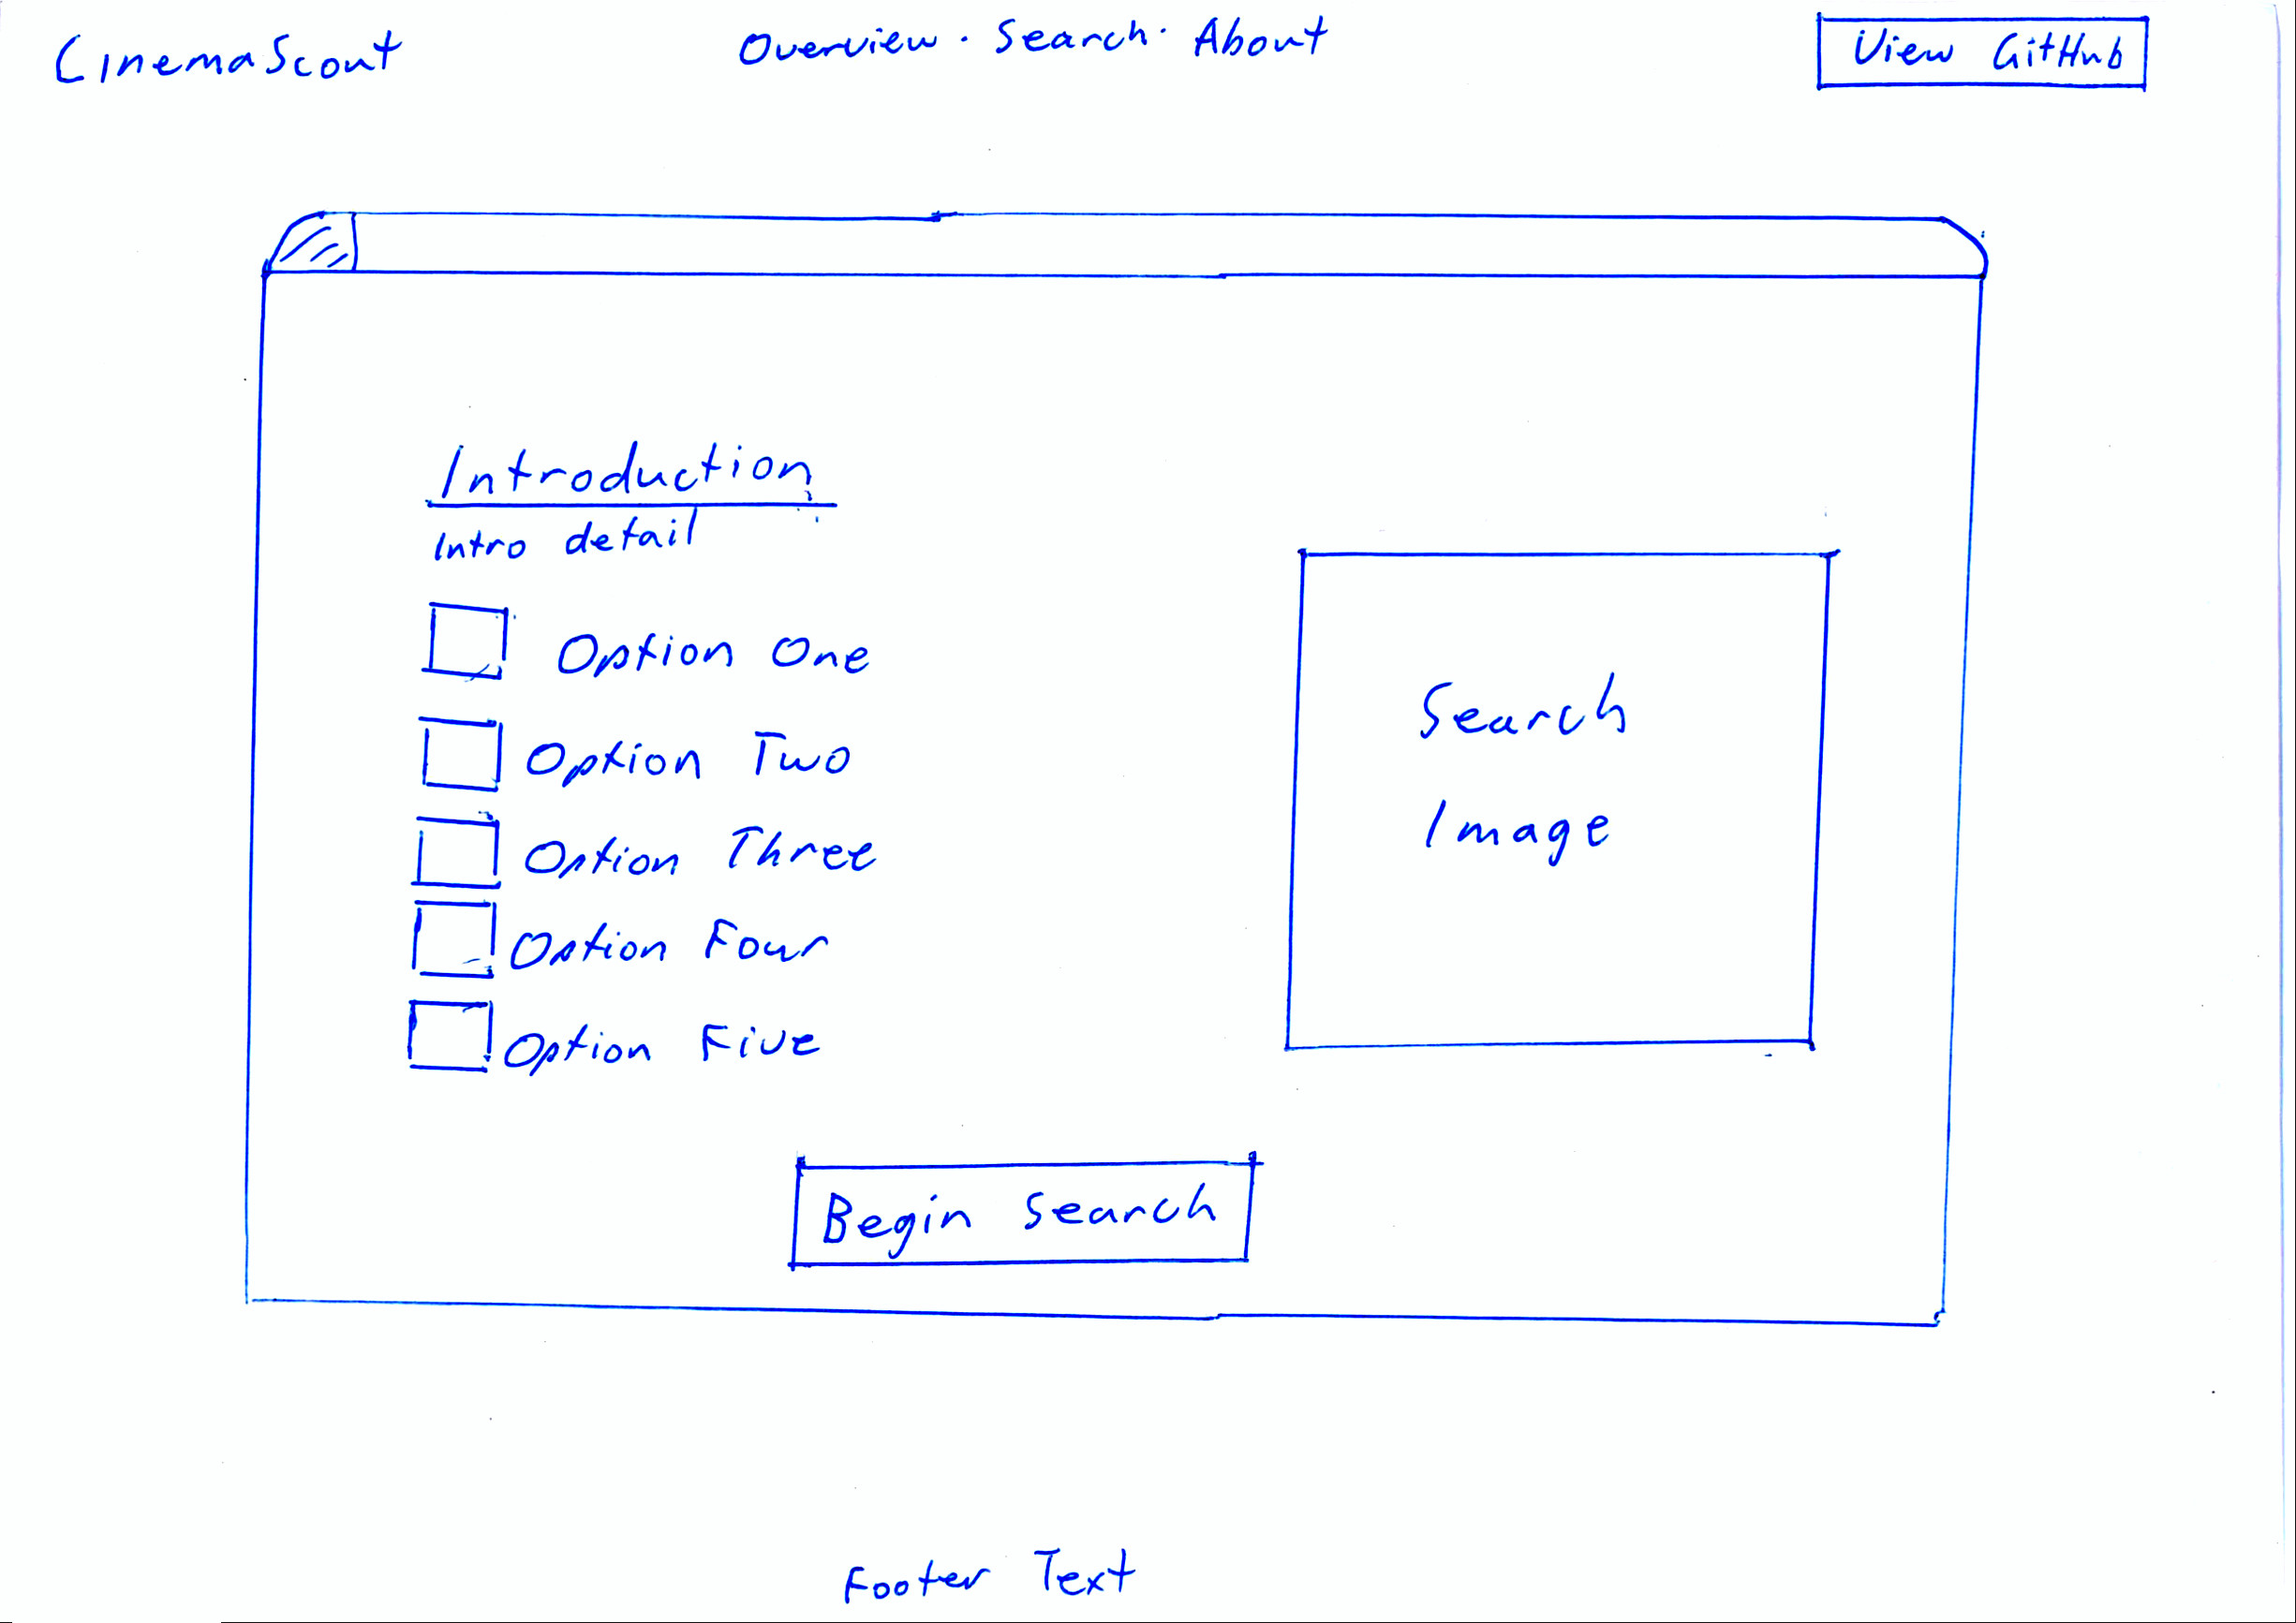
\includegraphics[width=\columnwidth]{res/search_begin.jpg}
\caption{Rough sketch of the initialise search state of the search page.}
\end{figure}
\begin{figure}[H]
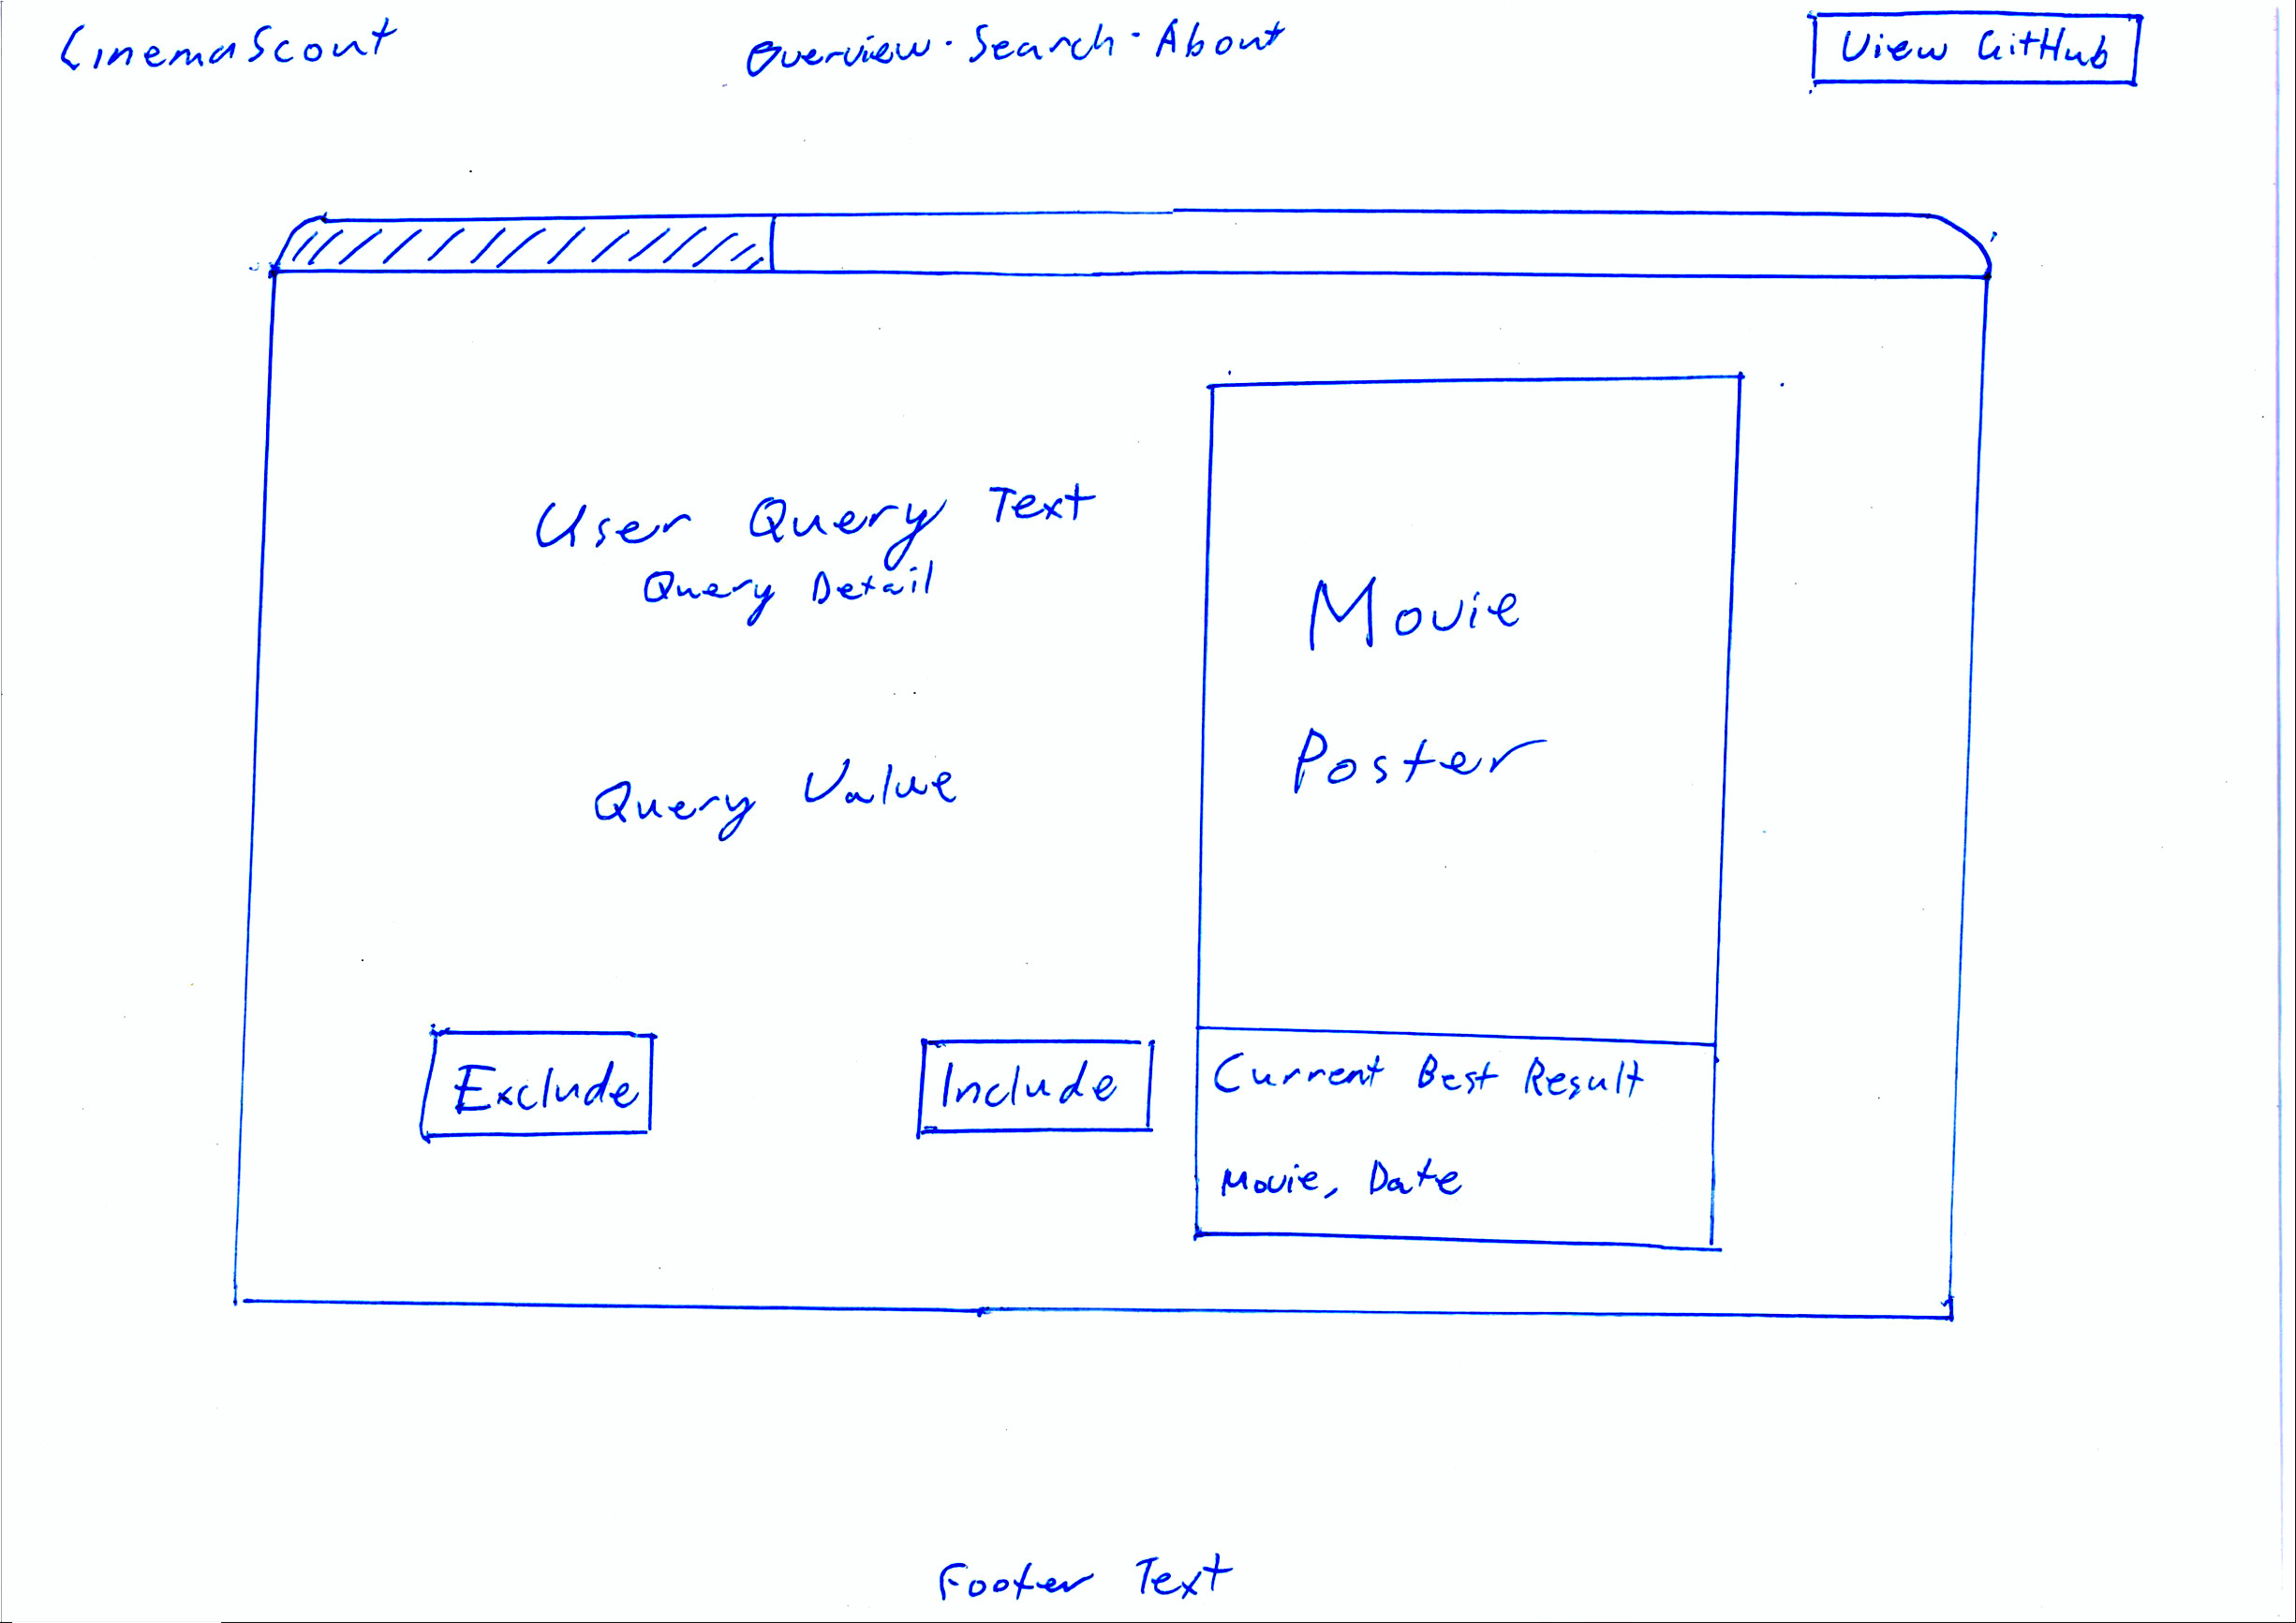
\includegraphics[width=\columnwidth]{res/search_next.jpg}
\caption{Rough sketch of the in progress state of the search page.}
\end{figure}
\subsection{About Page}
\begin{figure}[H]
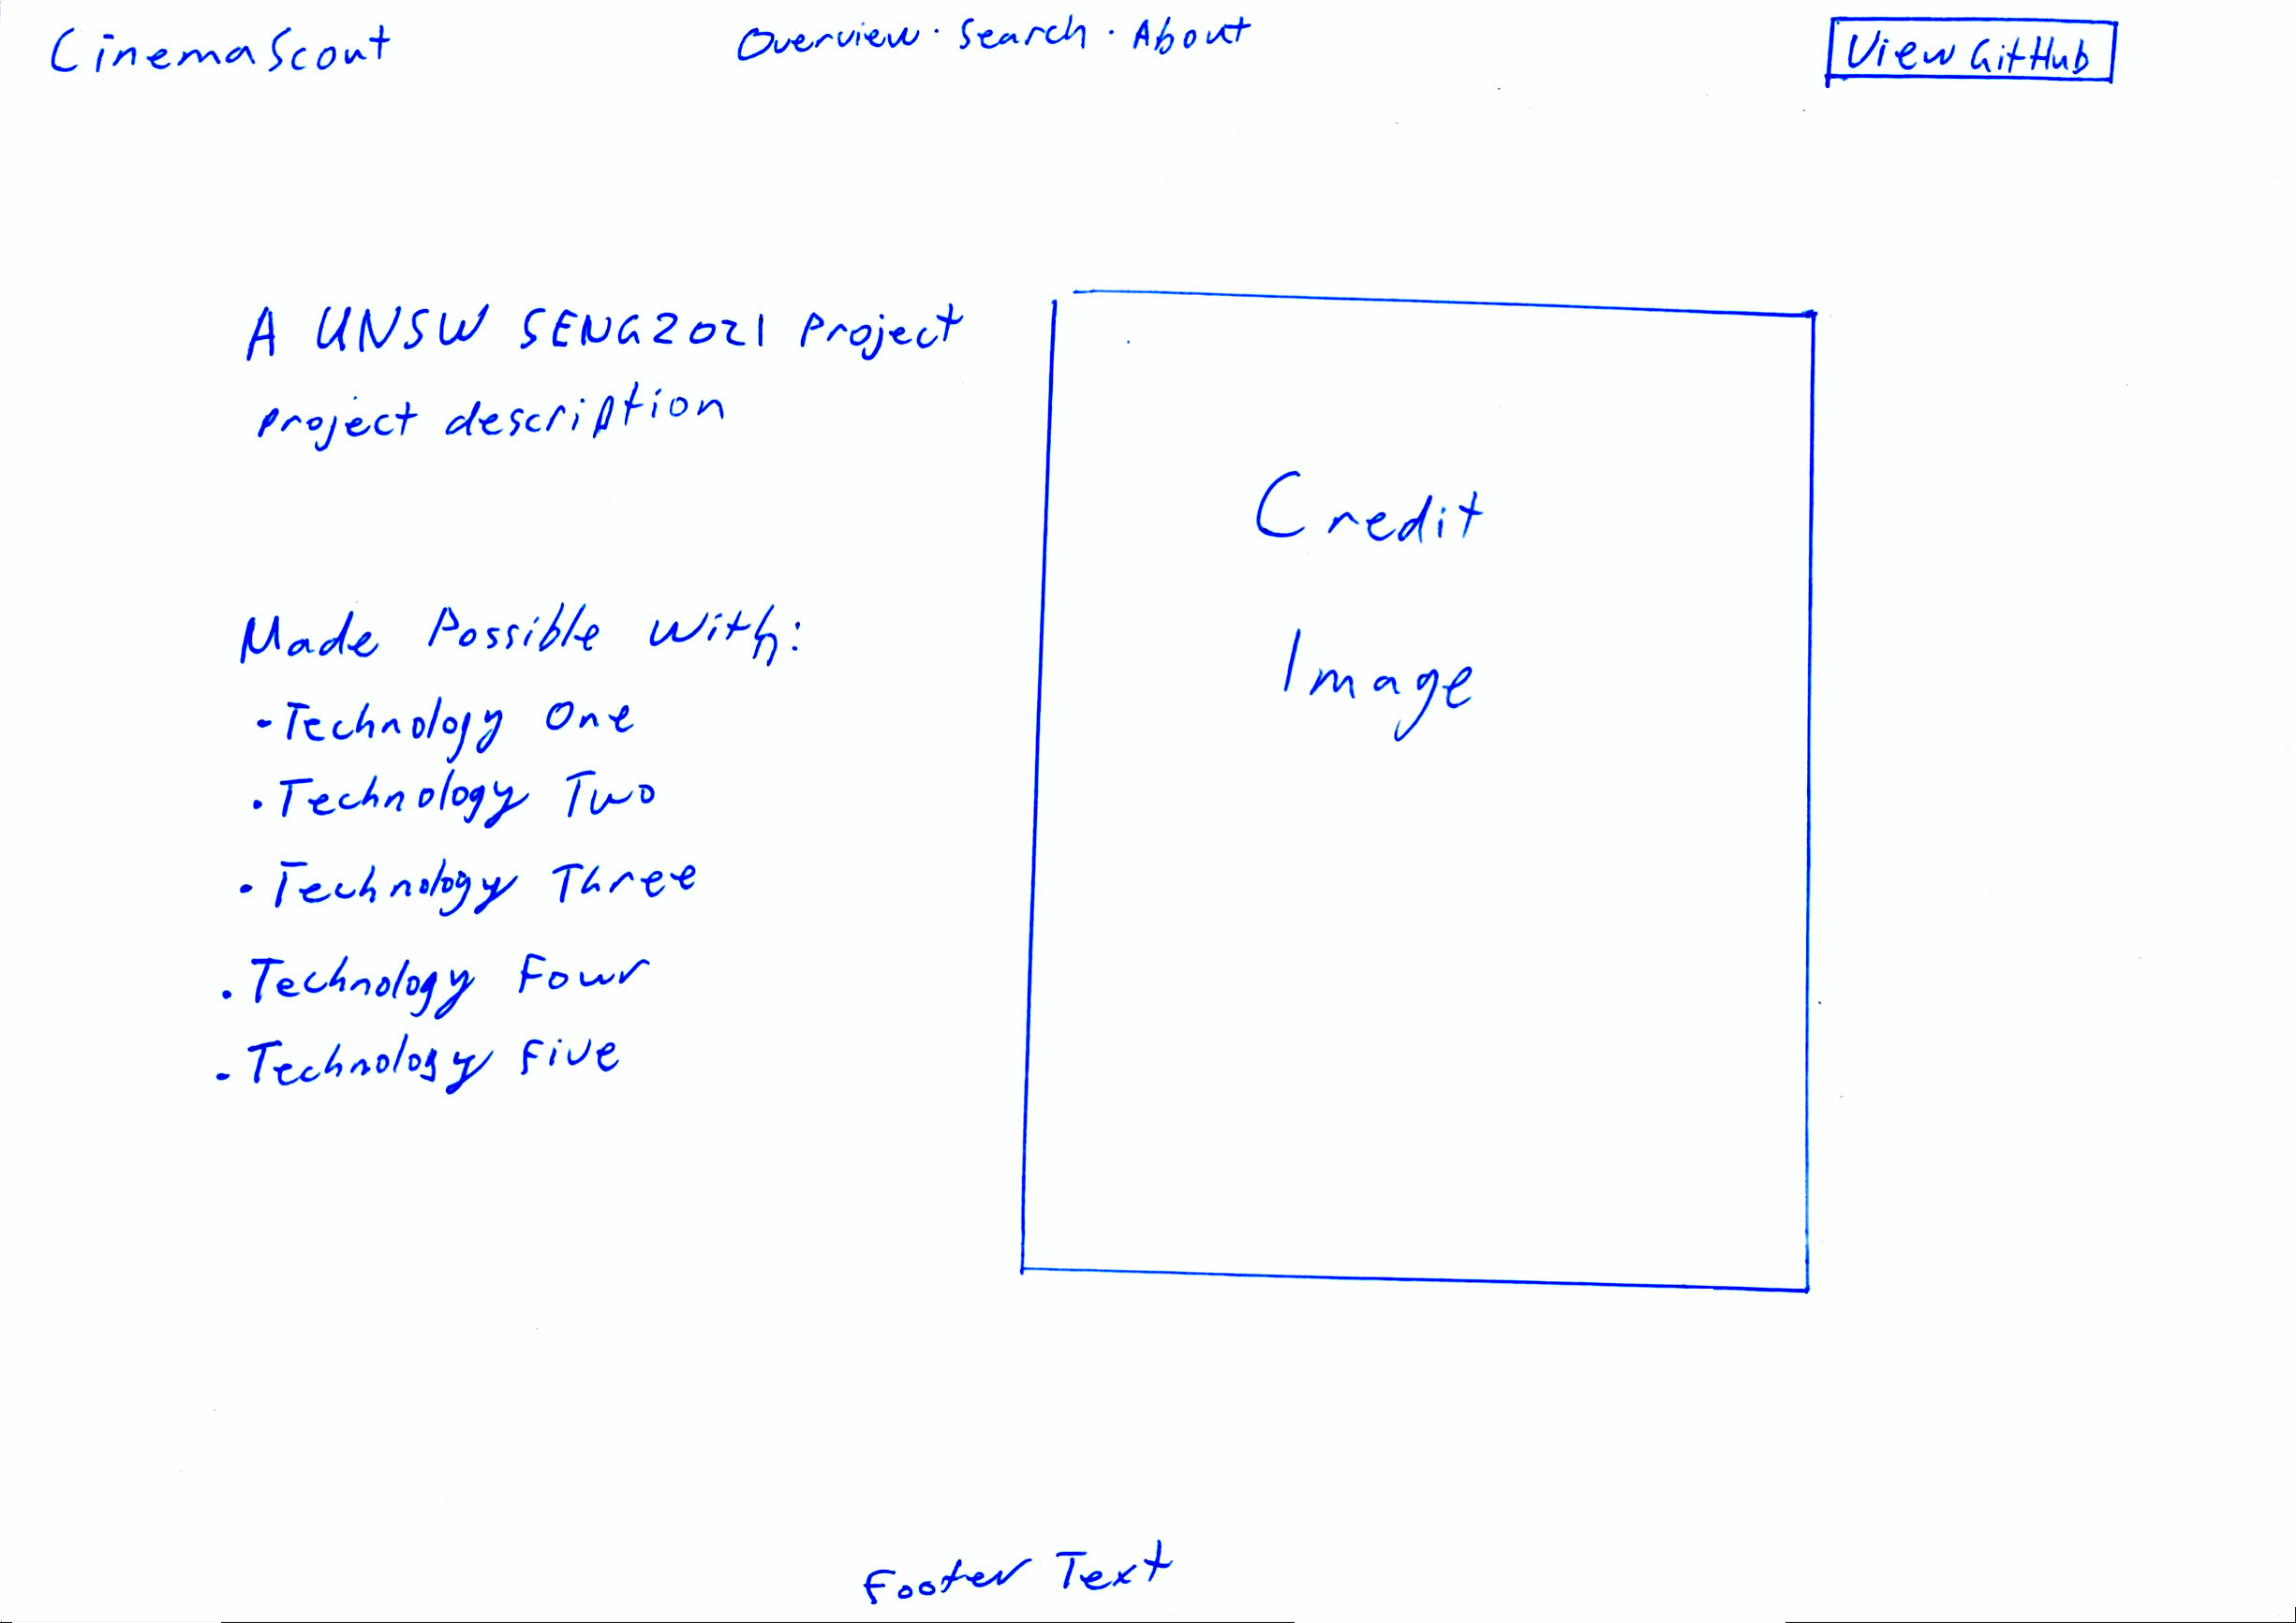
\includegraphics[width=\columnwidth]{res/credits.jpg}
\caption{Rough sketch of the about page.}
\end{figure}
\subsection{Storyboard Composite}
\begin{figure}[H]
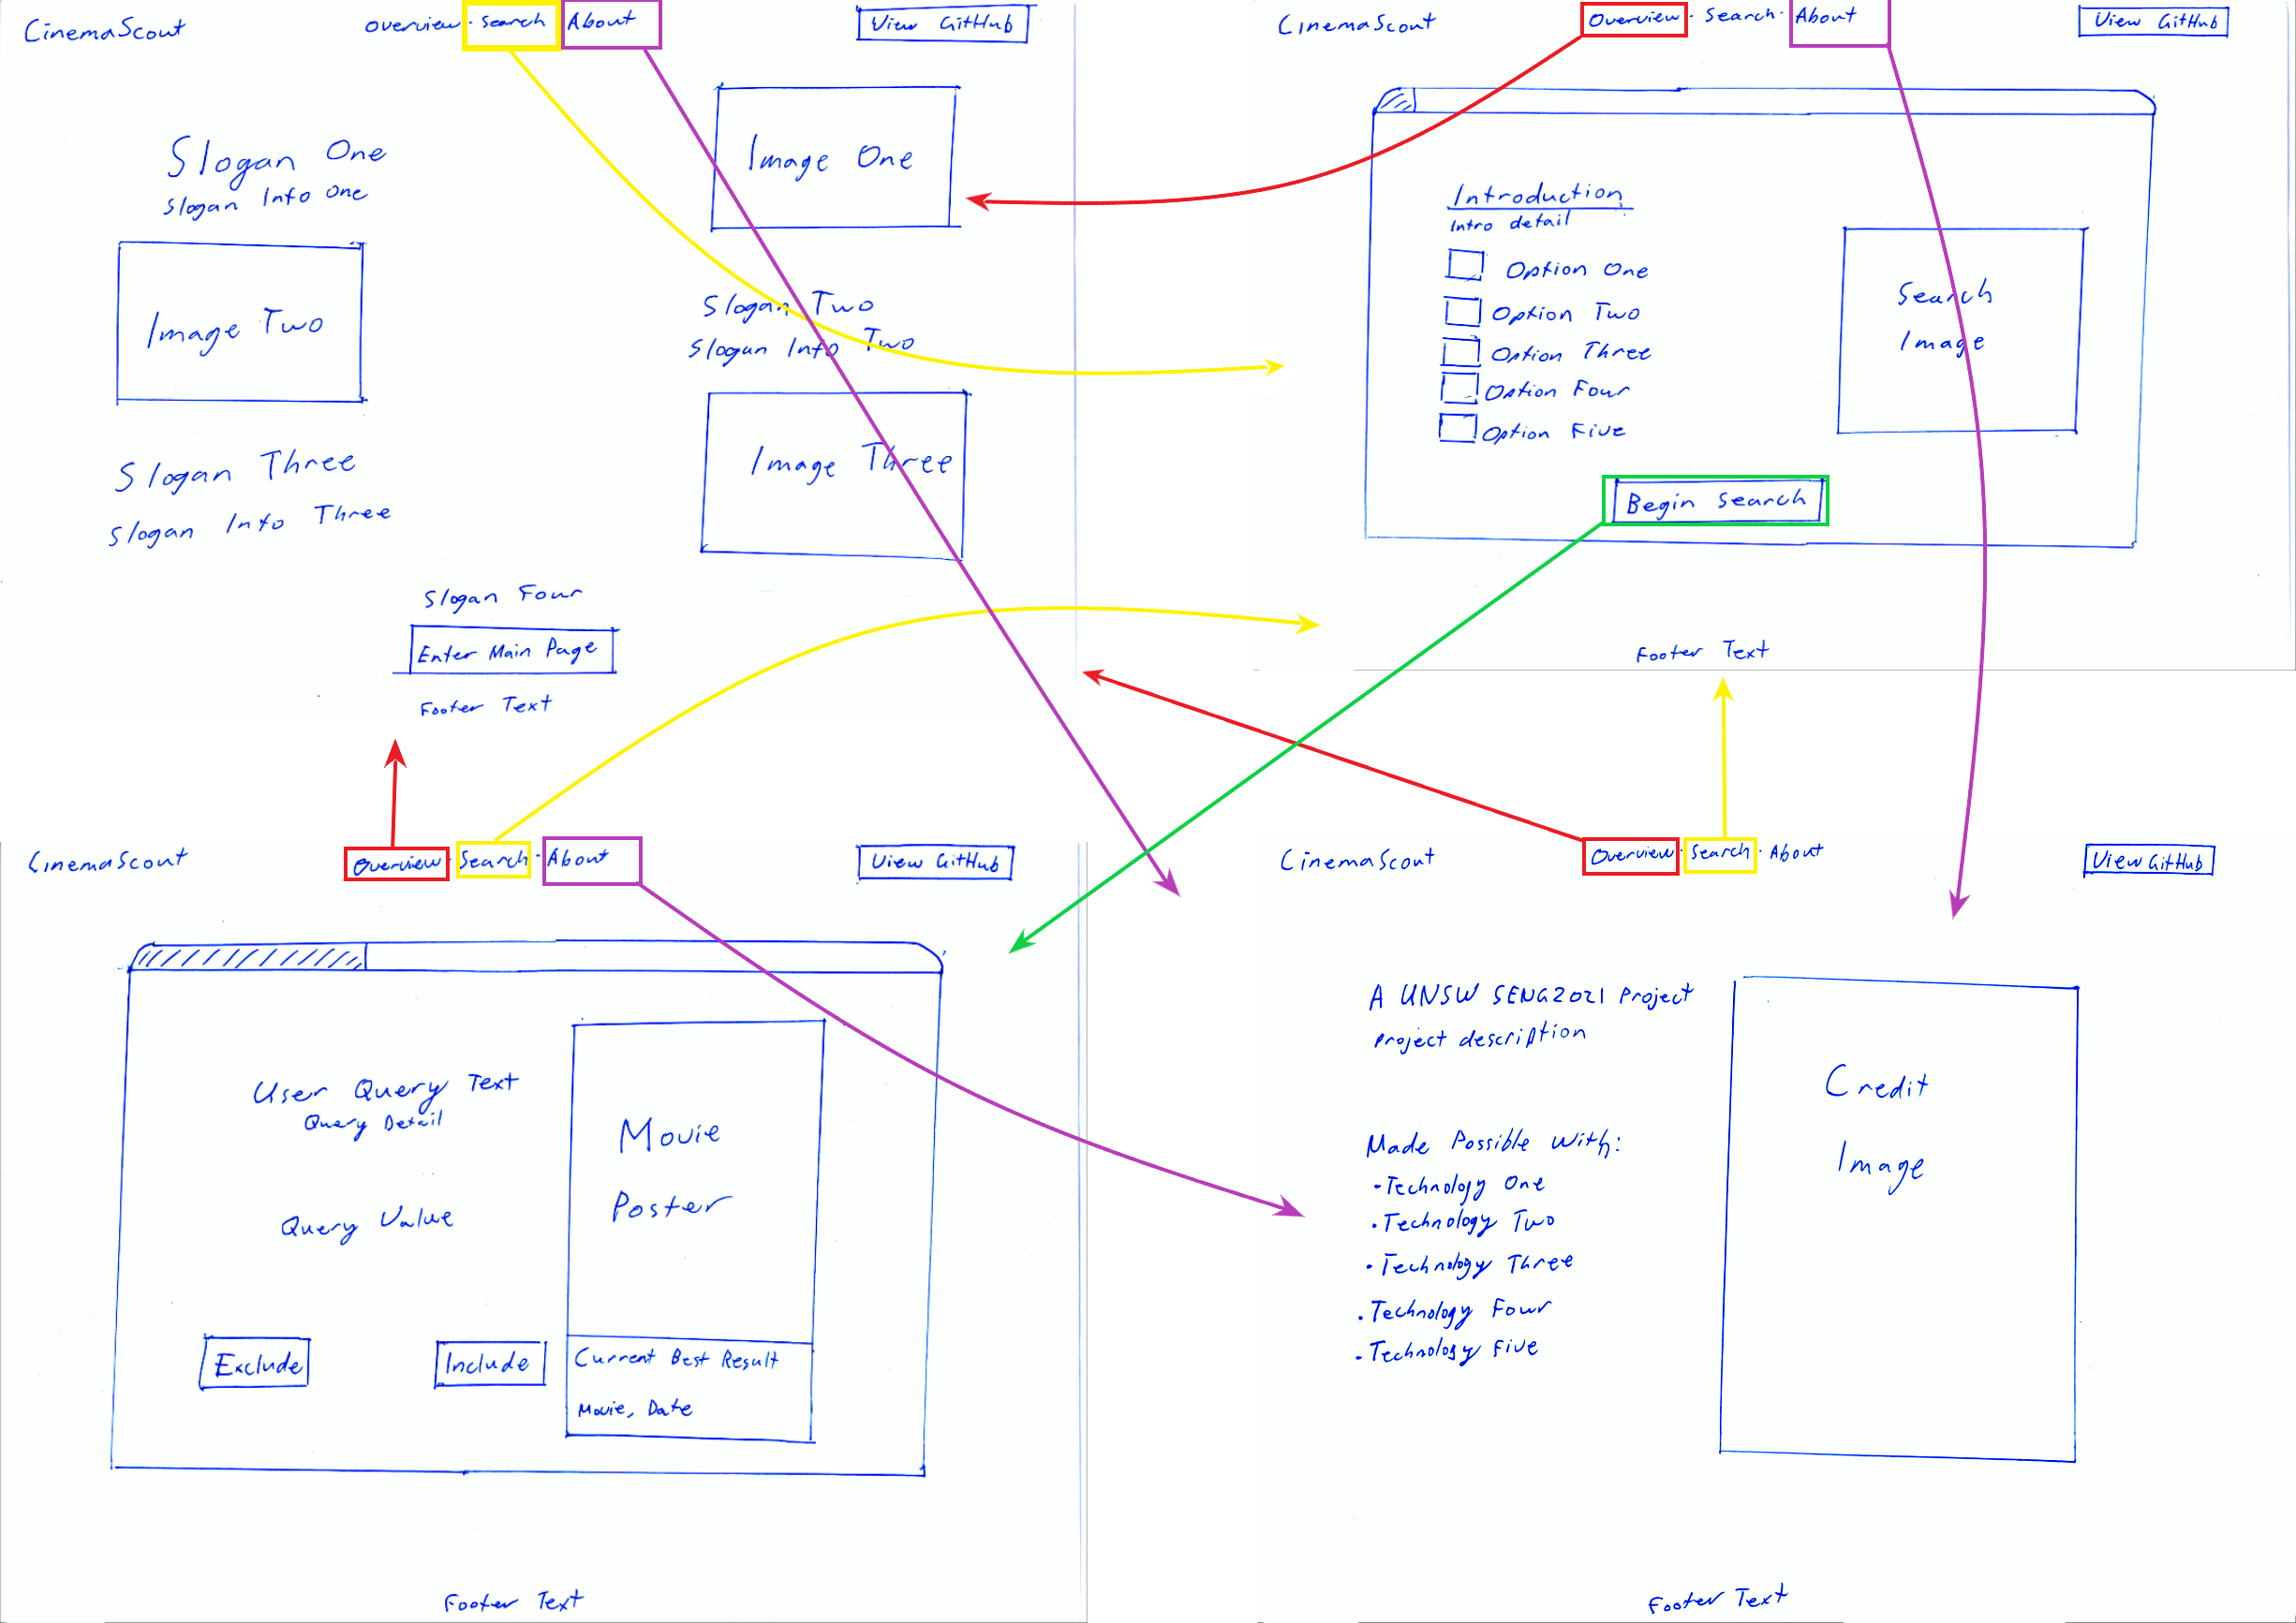
\includegraphics[width=\columnwidth]{res/arrows_new.png}
\caption{Storyboard sketch of all previous figures.}
\end{figure}

\section{High-Fiedelity Prototype}
The following images are a work in progress and do not represent the final
design of the product. All images were captured at a resolution of 1920 x
1080 using a default Chromium browser on Arch Linux. An interactable, 
high-fidelity prototype is available on GitHub.
\subsection{Landing Page}
\begin{figure}[H]
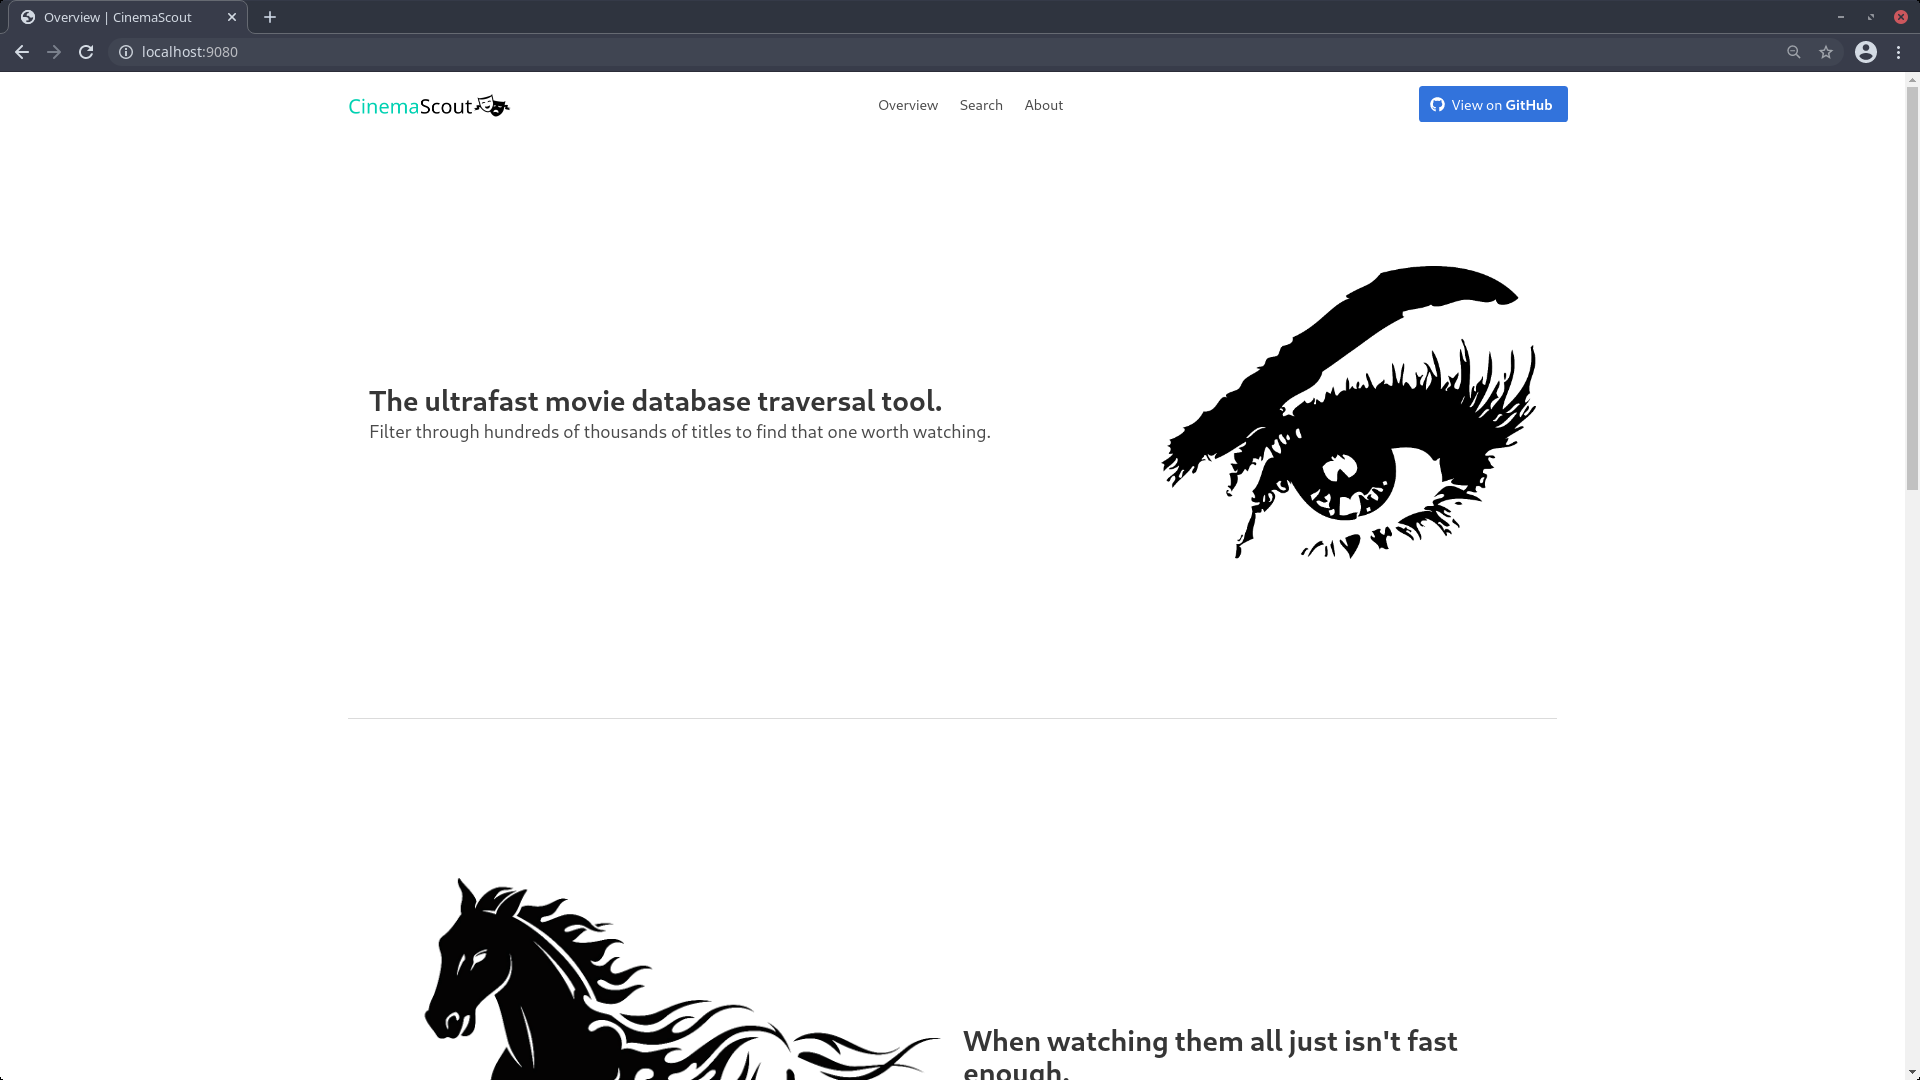
\includegraphics[width=\columnwidth]{res/landing_1.png}
\caption{Upper portion of the landing page.}
\end{figure}
\begin{figure}[H]
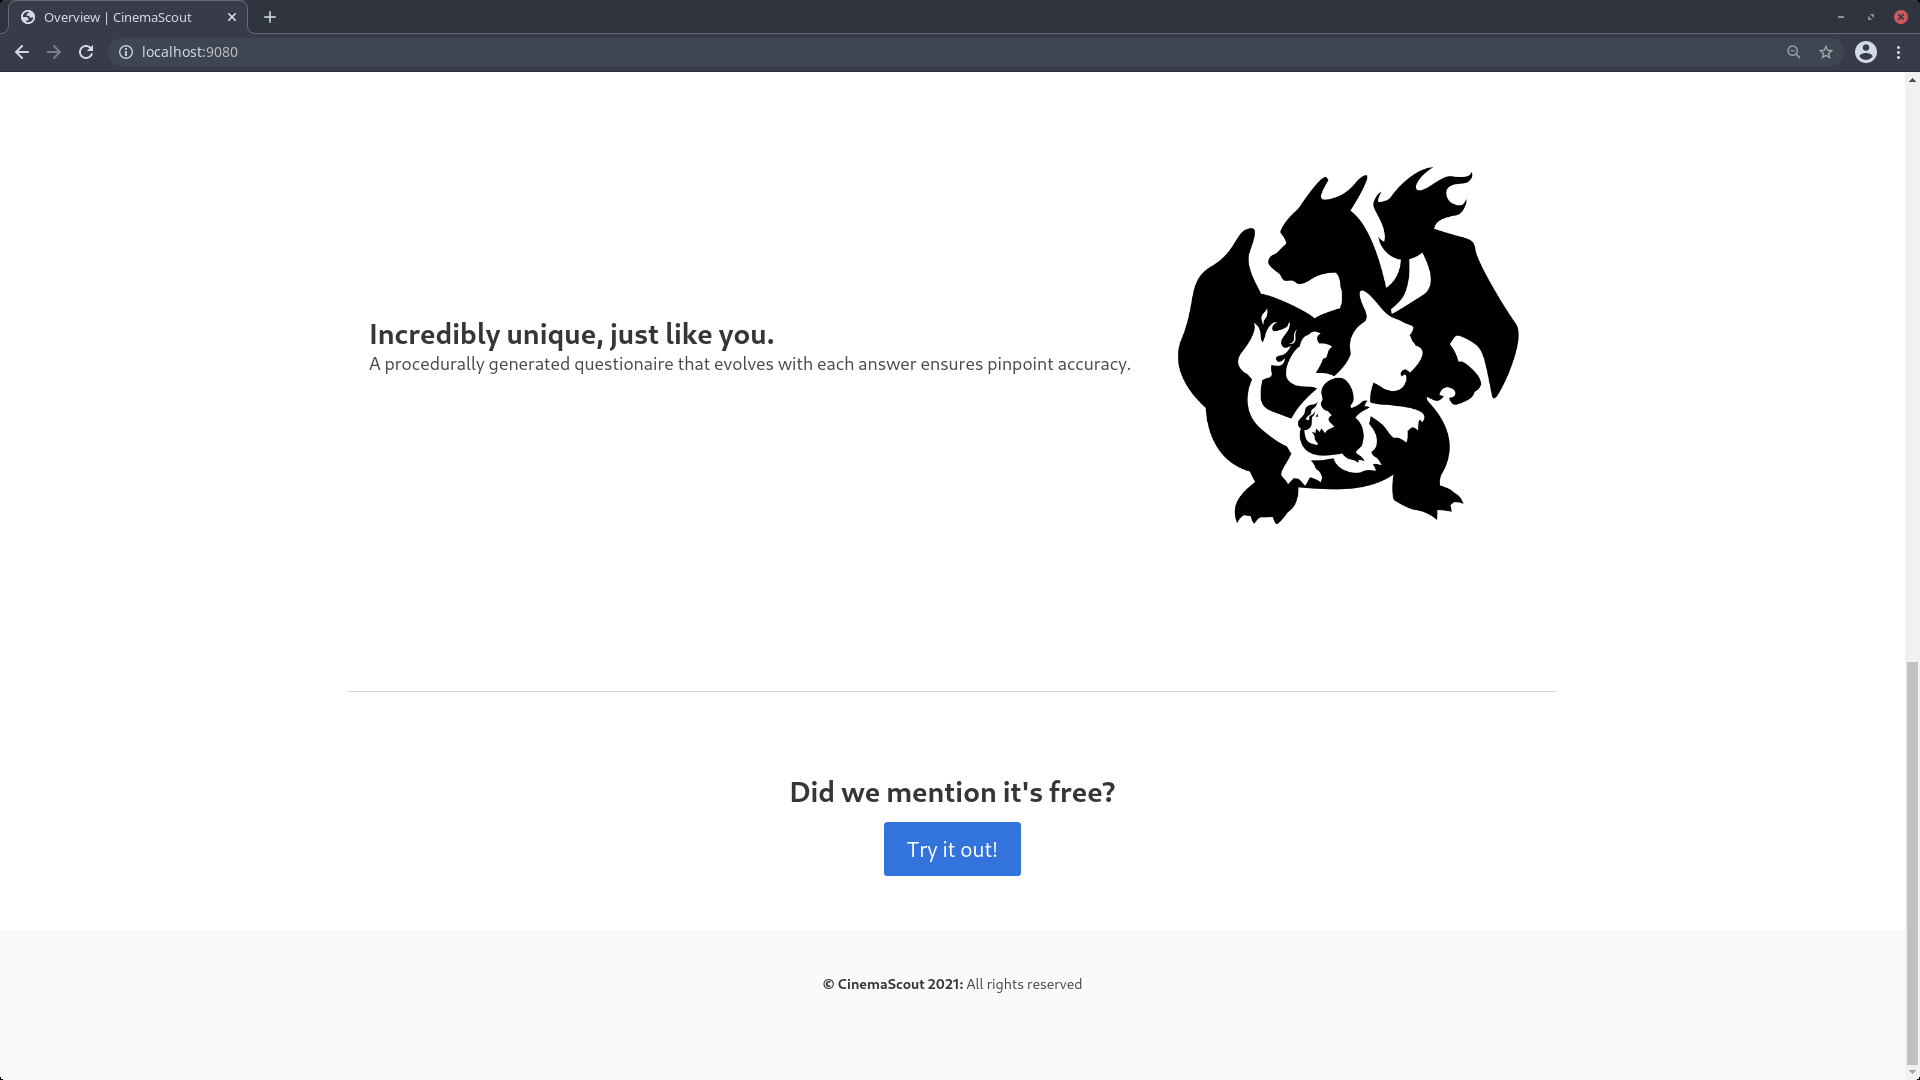
\includegraphics[width=\columnwidth]{res/landing_2.png}
\caption{Lower portion of the landing page.}
\end{figure}
\subsection{Search Page}
\begin{figure}[H]
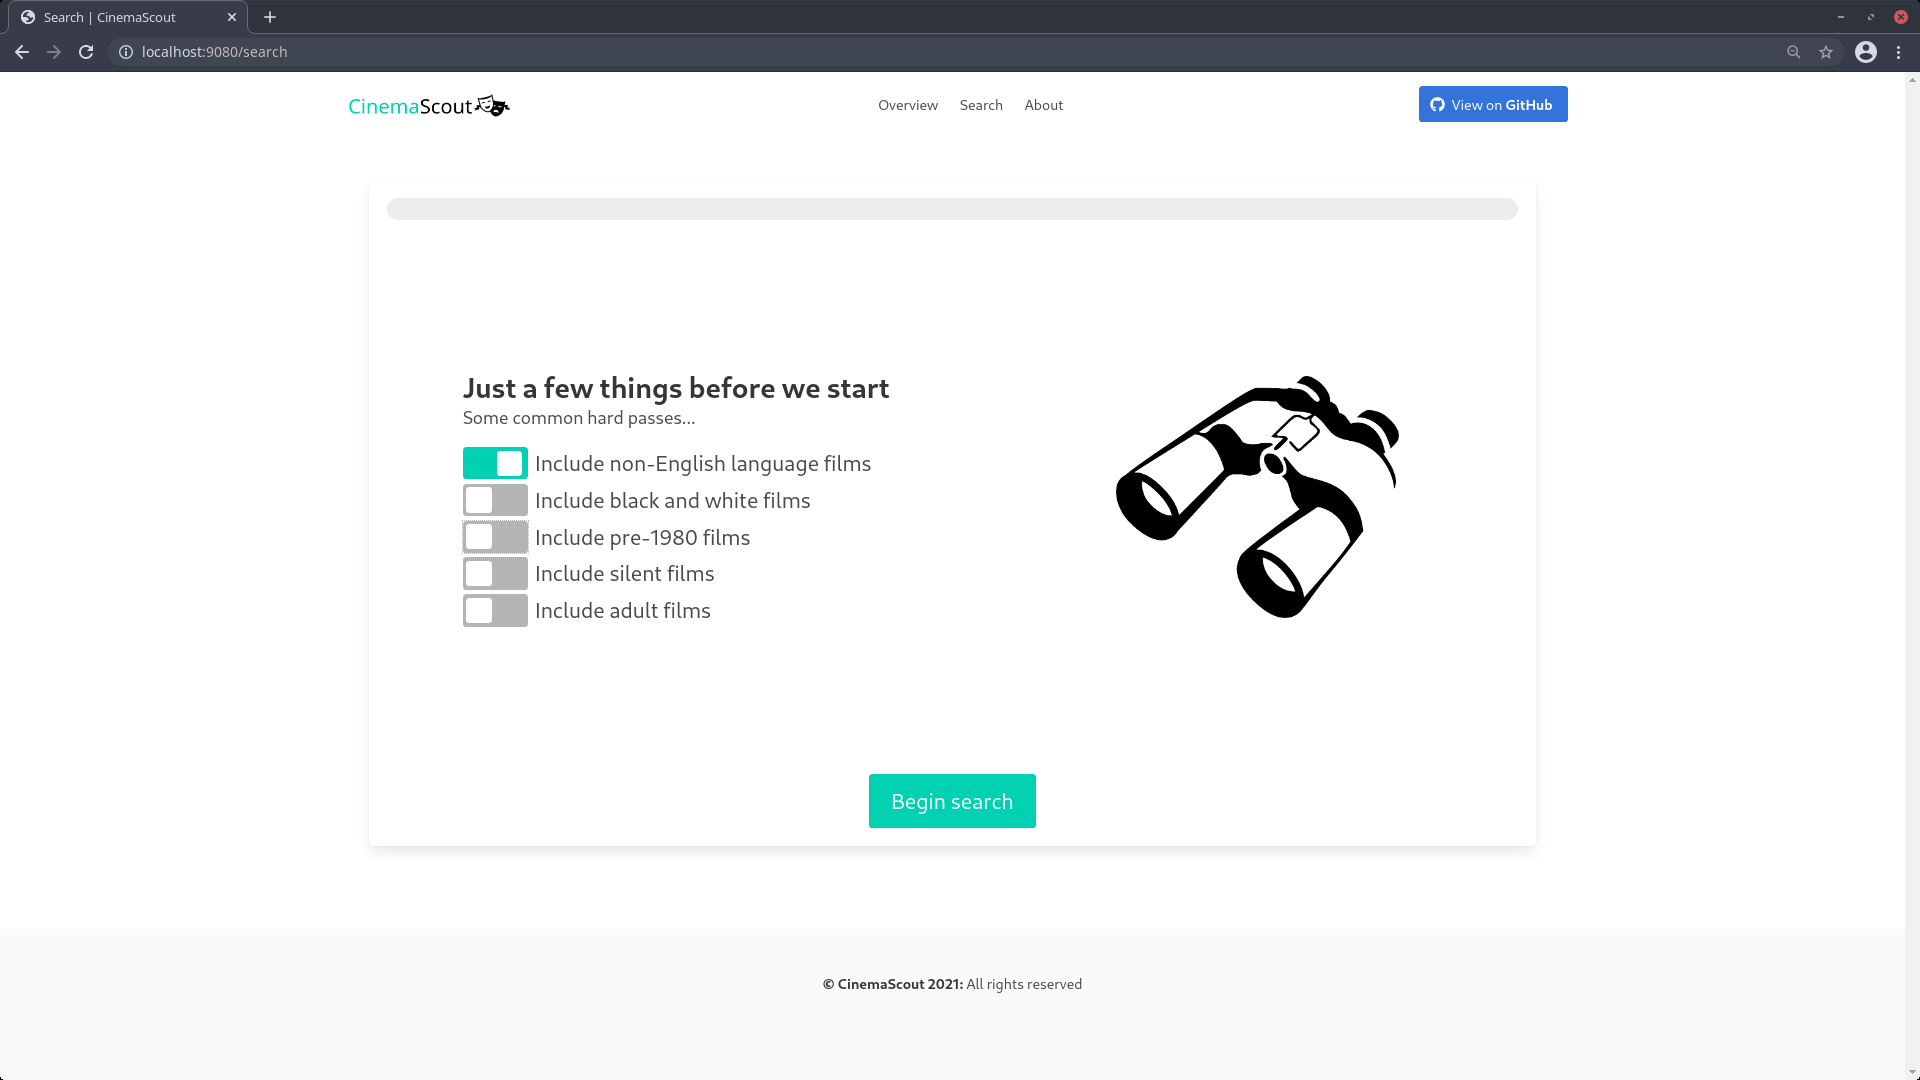
\includegraphics[width=\columnwidth]{res/search_1.png}
\caption{Initialise search state of the search page.}
\end{figure}
\begin{figure}[H]
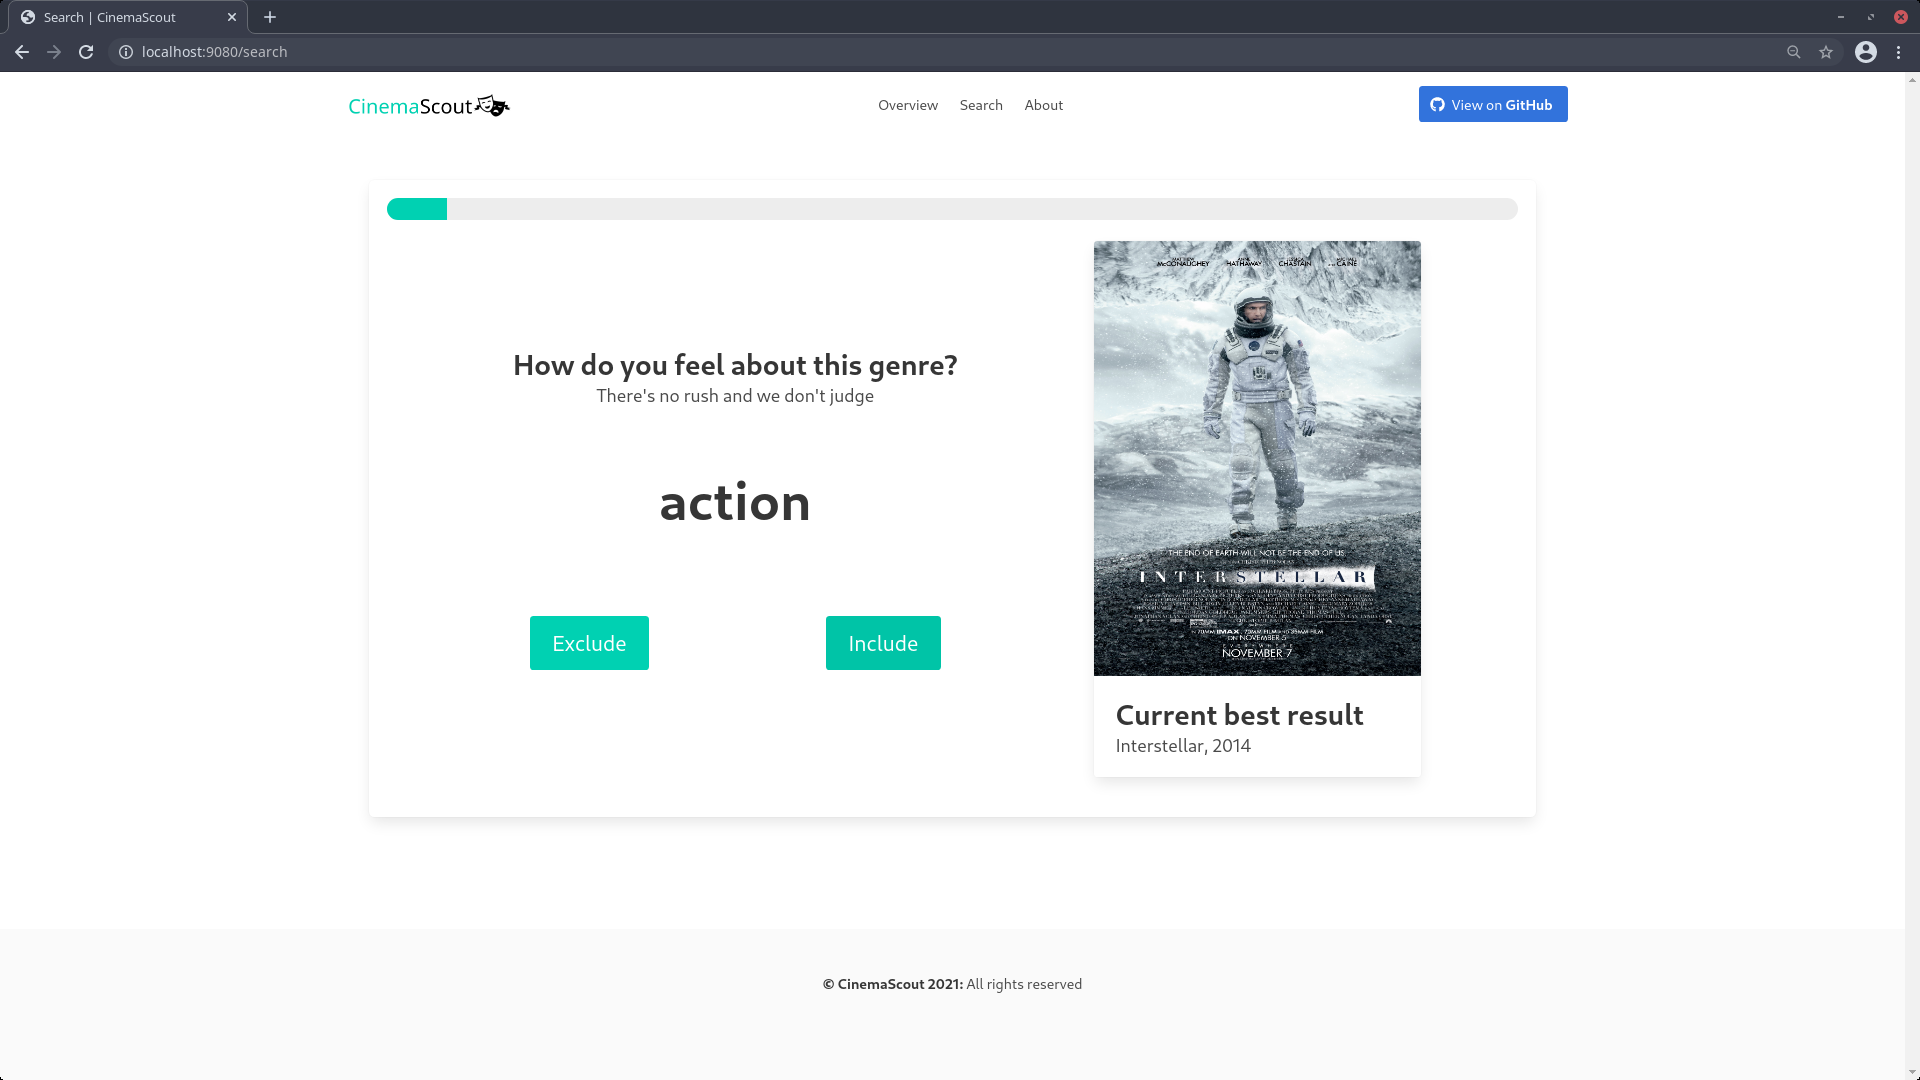
\includegraphics[width=\columnwidth]{res/search_2.png}
\caption{Search in progress state of the search page.}
\end{figure}
\subsection{About Page}
\begin{figure}[H]
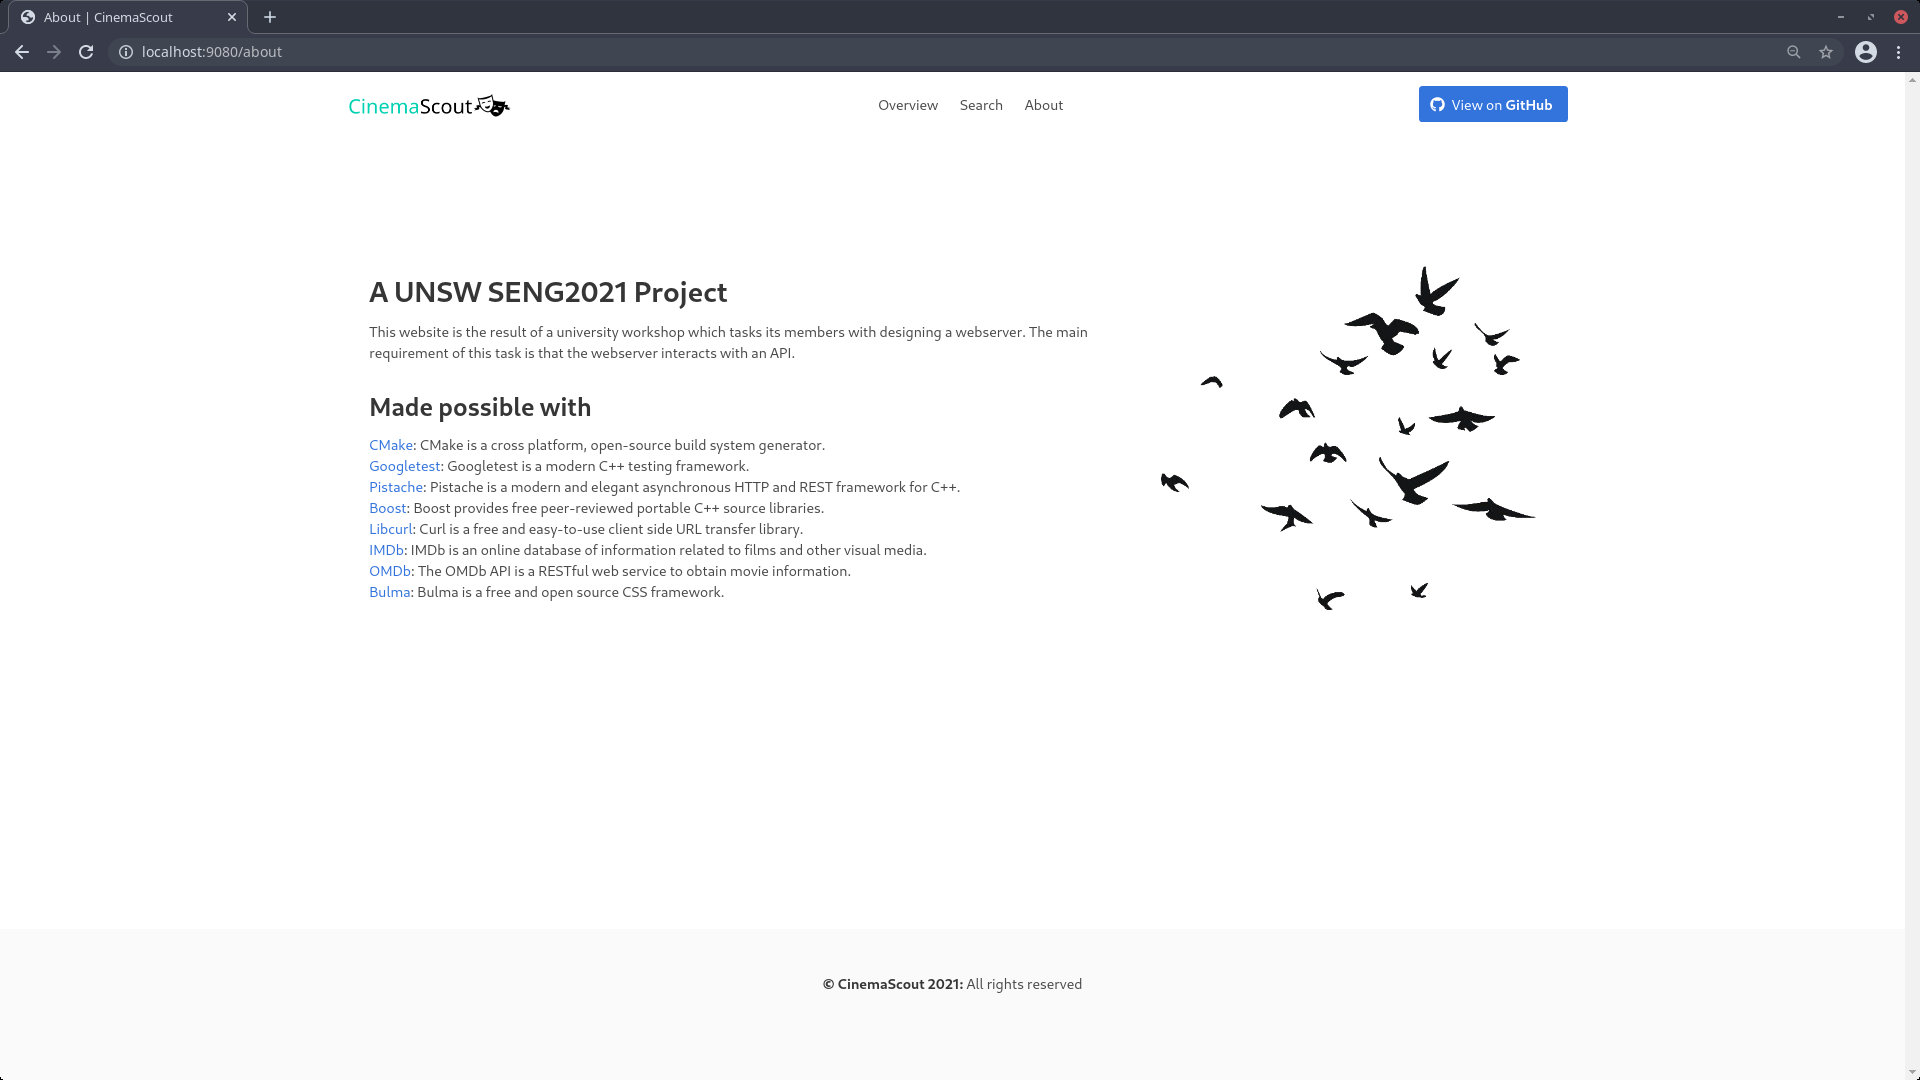
\includegraphics[width=\columnwidth]{res/about.png}
\caption{Entire portion of the about page.}
\end{figure}

\end{document}
